\documentclass[tikz,border=1pt]{standalone}
\usepackage[T1]{fontenc}
\usepackage{helvet}
\renewcommand{\familydefault}{\sfdefault}
\usepackage{amsmath,amssymb,bm}
\usetikzlibrary{positioning,patterns,arrows.meta,calc,fit,backgrounds}
\hyphenpenalty=10000 \exhyphenpenalty=10000
\definecolor{oiblue}{HTML}{0072B2}\definecolor{oiorange}{HTML}{E69F00}\definecolor{oigreen}{HTML}{009E73}
\definecolor{oiverm}{HTML}{D55E00}\definecolor{oipurple}{HTML}{CC79A7}\definecolor{oisky}{HTML}{56B4E9}
\definecolor{oigray}{HTML}{666666}
\newcommand{\fs}{\fontsize{7}{8.6}\selectfont}
\newcommand{\fss}{\fontsize{6.5}{7.5}\selectfont}
\tikzset{
  bx/.style={draw=#1, fill=#1!7, rounded corners=1.5pt, line width=0.5pt, align=center, inner sep=1.1mm, font=\fs},
  bx/.default=oigray,
  panel/.style={draw=oigray!60, line width=0.5pt, rounded corners=2pt, inner sep=1.6mm},
  ptitle/.style={font=\fontsize{9}{10}\selectfont\bfseries, anchor=north west, inner sep=0pt},
  arr/.style={-{Stealth[length=1.6mm]}, line width=0.6pt, draw=black!75},
}
\newcommand{\T}[1]{{\fontsize{8}{9.6}\selectfont\bfseries #1}\\[0.5mm]}
\newcommand{\stage}[1]{\tikz[baseline=-0.6ex]\node[draw=oigreen,fill=white,minimum width=4.2mm,minimum height=3mm,inner sep=0,font=\fss]{#1};}
% cell value v (1,0,?) at lower-left (x,y)
\newcommand{\cell}[3]{%
  \if1#3\fill[oiblue] (#1,#2) rectangle ++(0.48,0.26); \node[white,font=\fss] at ($(#1,#2)+(0.24,0.13)$) {1};\fi
  \if0#3\draw[oigray!70,line width=0.4pt] (#1,#2) rectangle ++(0.48,0.26); \node[oigray,font=\fss] at ($(#1,#2)+(0.24,0.13)$) {0};\fi
  \if?#3\fill[pattern=north east lines,pattern color=oigray!55] (#1,#2) rectangle ++(0.48,0.26);
        \draw[oigray!70,line width=0.4pt] (#1,#2) rectangle ++(0.48,0.26);
        \node[font=\fss\bfseries] at ($(#1,#2)+(0.24,0.13)$) {?};\fi}
\newcommand{\dbrow}[3]{% top-y, row index, list
  \node[font=\fss] at (0.5,#1-0.95-0.33*#2) {R\the\numexpr#2+1\relax};
  \foreach \v [count=\i from 0] in {#3} {\cell{0.9+0.6*\i}{#1-1.08-0.33*#2}{\v}}}
\newcommand{\db}[5]{% top-y, title, three rows
  \draw[oigray!80, line width=0.5pt, rounded corners=1.5pt] (0.15,#1) rectangle (4.05,#1-2.0);
  \node[font=\fontsize{8}{9.6}\selectfont\bfseries, anchor=north] at (2.1,#1-0.07) {#2};
  \foreach \h [count=\i from 0] in {AF,RBBB,LAD,TInv,Brady} \node[font=\fss] at (1.14+0.6*\i,#1-0.62) {\h};
  \dbrow{#1}{0}{#3}\dbrow{#1}{1}{#4}\dbrow{#1}{2}{#5}}

\begin{document}
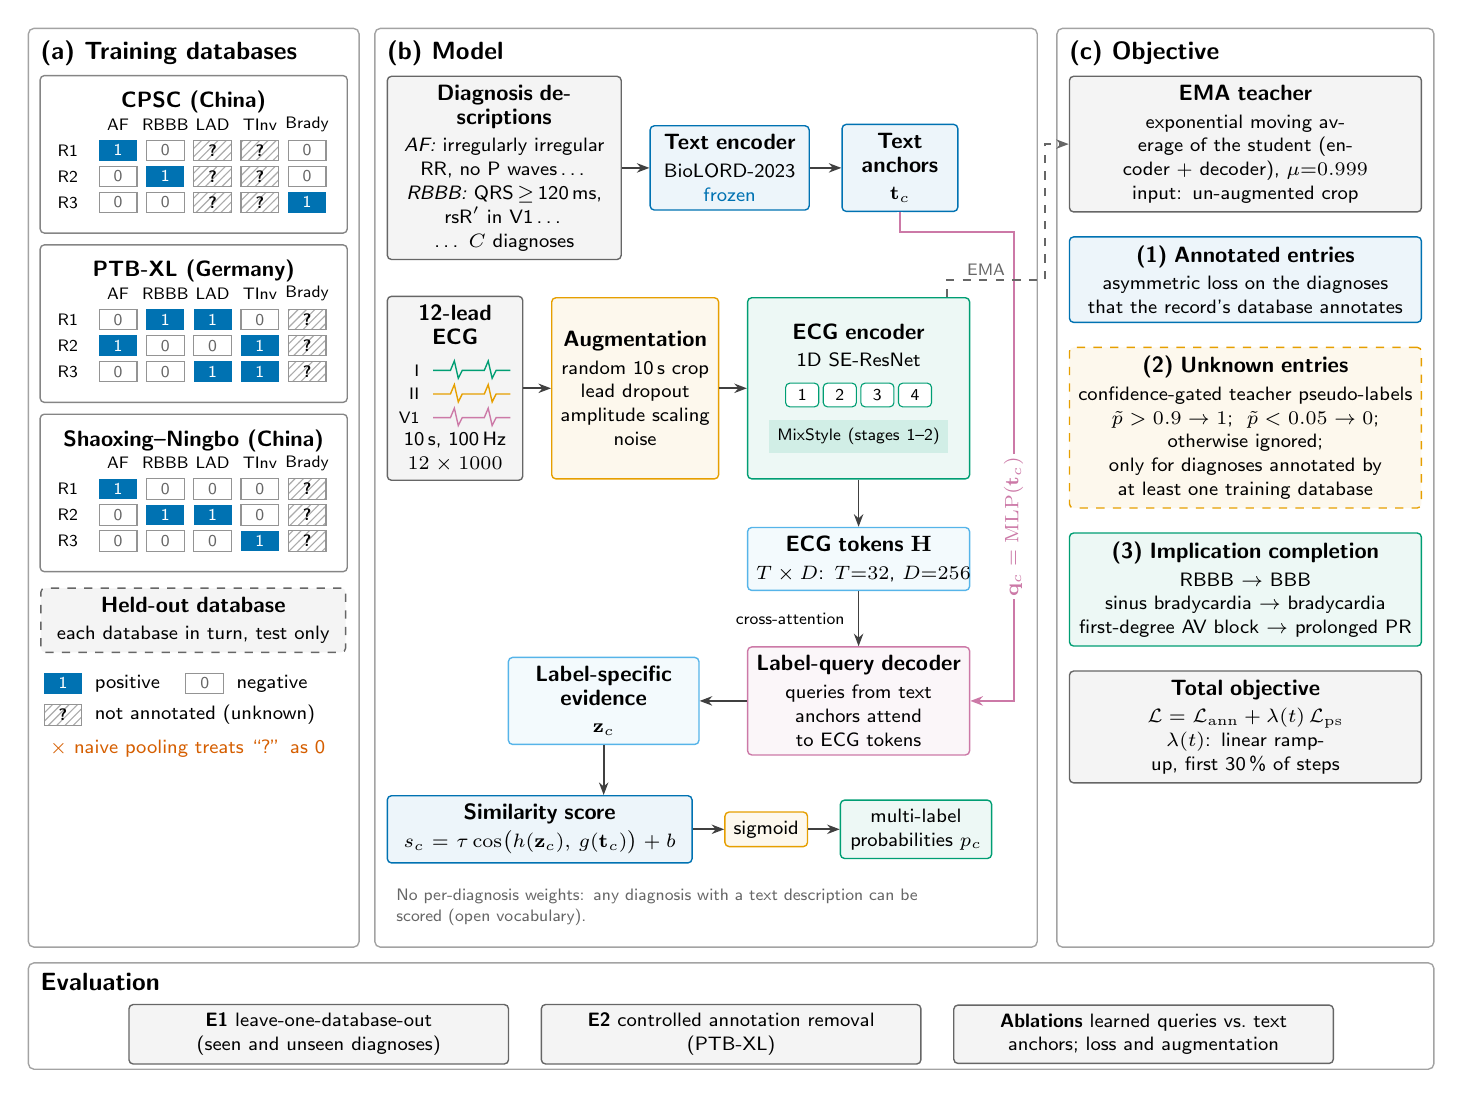
\begin{tikzpicture}[x=1cm,y=1cm, node distance=3mm]
%======================== (a)
\node[ptitle] (ta) at (0.15,-0.15) {(a) Training databases};
\db{-0.6}{CPSC (China)}{1,0,?,?,0}{0,1,?,?,0}{0,0,?,?,1}
\db{-2.75}{PTB-XL (Germany)}{0,1,1,0,?}{1,0,0,1,?}{0,0,1,1,?}
\db{-4.9}{Shaoxing--Ningbo (China)}{1,0,0,0,?}{0,1,1,0,?}{0,0,0,1,?}
\node[bx, dashed, text width=3.65cm, anchor=north west] (held) at (0.15,-7.1) {\T{Held-out database}each database in turn, test only};
\cell{0.2}{-8.45}{1}\node[anchor=west,font=\fs] at (0.72,-8.32) {positive};
\cell{2.0}{-8.45}{0}\node[anchor=west,font=\fs] at (2.52,-8.32) {negative};
\cell{0.2}{-8.85}{?}\node[anchor=west,font=\fs] at (0.72,-8.72) {not annotated (unknown)};
\node[anchor=west,font=\fs, text=oiverm] (naive) at (0.15,-9.15) {\textbf{$\times$} naive pooling treats ``?'' as 0};
\coordinate (aR) at (4.2,0);

%======================== (b)
\node[ptitle] (tb) at (4.55,-0.15) {(b) Model};
\node[bx, text width=2.75cm, anchor=north west] (desc) at (4.55,-0.6)
  {\T{Diagnosis descriptions}\emph{AF:} irregularly irregular RR, no P waves\,\ldots\\ \emph{RBBB:} QRS\,$\geq$\,120\,ms, rsR$'$ in V1\,\ldots\\ \ldots\ $C$ diagnoses};
\node[bx=oiblue, text width=1.8cm, right=3.5mm of desc] (tenc) {\T{Text encoder}BioLORD-2023\\ \textcolor{oiblue}{frozen}};
\node[bx=oiblue, text width=1.25cm, right=4mm of tenc] (anch) {\T{Text anchors}$\mathbf{t}_c$};
\draw[arr] (desc) -- (tenc); \draw[arr] (tenc) -- (anch);

\node[bx, text width=1.5cm, anchor=north west, minimum height=2.3cm] (ecg) at ($(desc.south west)+(0,-0.45)$)
  {\T{12-lead ECG}\rule{0pt}{9mm}\\ 10\,s, 100\,Hz\\ $12\times1000$};
\begin{scope}[shift={($(ecg.north west)+(0.42,-0.95)$)}]
  \foreach \l/\c/\yy in {I/oigreen/0,II/oiorange/-0.3,V1/oipurple/-0.6} {
    \node[font=\fss, anchor=east] at (0.12,\yy) {\l};
    \draw[\c, line width=0.5pt] (0.17,\yy) -- ++(0.22,0) -- ++(0.05,0.12) -- ++(0.05,-0.22) -- ++(0.05,0.1)
      -- ++(0.28,0) -- ++(0.05,0.12) -- ++(0.05,-0.22) -- ++(0.05,0.1) -- ++(0.18,0);}
\end{scope}
\node[bx=oiorange, text width=1.9cm, minimum height=2.3cm, right=3.5mm of ecg] (aug)
  {\T{Augmentation}random 10\,s crop\\ lead dropout\\ amplitude scaling\\ noise};
\node[bx=oigreen, text width=2.6cm, minimum height=2.3cm, right=3.5mm of aug] (enc)
  {\T{ECG encoder}1D SE-ResNet\\[1.2mm] \stage{1}\,\stage{2}\,\stage{3}\,\stage{4}\\[1.2mm]
   \colorbox{oigreen!18}{\fss MixStyle (stages 1--2)}};
\draw[arr] (ecg) -- (aug); \draw[arr] (aug) -- (enc);

\node[bx=oisky, text width=2.6cm, below=6mm of enc] (tok) {\T{ECG tokens $\mathbf{H}$}\mbox{$T\times D$: $T{=}32$, $D{=}256$}};
\draw[arr] (enc) -- (tok);
\node[bx=oipurple, text width=2.6cm, below=7mm of tok] (dec) {\T{Label-query decoder}queries from text anchors attend to ECG tokens};
\draw[arr] (tok) -- node[left, font=\fss, xshift=-0.5mm] {cross-attention} (dec);
\node[bx=oisky, text width=2.2cm, left=6mm of dec] (evi) {\T{Label-specific evidence}$\mathbf{z}_c$};
\draw[arr] (dec) -- (evi);
% text anchors -> label queries (right-hand column)
\coordinate (qx) at ($(enc.east)+(0.55,0)$);
\draw[arr, draw=oipurple, line width=0.8pt, preaction={draw=white,line width=2.4pt}] (anch.south) |- ($(anch.south)+(0,-0.25)$) -| (qx|-dec.east) -- (dec.east);
\node[font=\fs, text=oipurple, rotate=90, fill=white, inner sep=1pt] at (qx|-tok.north) {$\mathbf{q}_c=\mathrm{MLP}(\mathbf{t}_c)$};

\node[bx=oiblue, text width=3.65cm, anchor=north west] (sim) at ($(ecg.south west|-dec.south)+(0,-0.5)$)
  {\T{Similarity score}$s_c=\tau\cos\!\big(h(\mathbf{z}_c),\,g(\mathbf{t}_c)\big)+b$};
\draw[arr] (evi.south) -- (evi.south|-sim.north);
\node[bx=oiorange, right=4mm of sim] (sig) {sigmoid};
\node[bx=oigreen, text width=1.7cm, right=4mm of sig] (prob) {multi-label\\ probabilities $p_c$};
\draw[arr] (sim) -- (sig); \draw[arr] (sig) -- (prob);
\node[font=\fss, text=oigray, below=2mm of sim.south west, anchor=north west, text width=7.2cm, align=left] (note)
  {No per-diagnosis weights: any diagnosis with a text description can be scored (open vocabulary).};

%======================== (c)
\coordinate (cx) at ($(qx)+(0.7,0)$);
\node[ptitle] (tc) at (cx|-tb.north) {(c) Objective};
\node[bx, text width=4.25cm, anchor=north west] (tea) at (cx|-desc.north)
  {\T{EMA teacher}exponential moving average of the student (encoder + decoder), \mbox{$\mu{=}0.999$}\\ input: un-augmented crop};
\node[bx=oiblue, text width=4.25cm, below=3mm of tea] (l1)
  {\T{(1) Annotated entries}asymmetric loss on the diagnoses that the record's database annotates};
\node[bx=oiorange, dashed, text width=4.25cm, below=3mm of l1] (l2)
  {\T{(2) Unknown entries}confidence-gated teacher pseudo-labels\\ \mbox{$\tilde p>0.9 \rightarrow 1$;\ \ $\tilde p<0.05\rightarrow 0$;}\ otherwise ignored;\\
   only for diagnoses annotated by at least one training database};
\node[bx=oigreen, text width=4.25cm, below=3mm of l2] (l3)
  {\T{(3) Implication completion}RBBB $\rightarrow$ BBB\\ sinus bradycardia $\rightarrow$ bradycardia\\ first-degree AV block $\rightarrow$ prolonged PR};
\node[bx, text width=4.25cm, below=3mm of l3] (tot)
  {\T{Total objective}\mbox{$\mathcal{L}=\mathcal{L}_{\mathrm{ann}}+\lambda(t)\,\mathcal{L}_{\mathrm{ps}}$}\\ $\lambda(t)$: linear ramp-up, first 30\,\% of steps};
% student -> teacher
\coordinate (S) at ($(enc.north east)+(-0.3,0)$); \coordinate (Y) at ($(enc.north east)+(0,0.22)$);
\coordinate (X) at ($(cx)+(-0.3,0)$);
\draw[arr, dashed, draw=oigray] (S) -- (S |- Y) -- (X |- Y) -- (X |- tea.west) -- (tea.west);
\node[font=\fss, text=oigray, fill=white, inner sep=0.6pt, anchor=south] at ($(enc.north east)+(0.2,0.24)$) {EMA};

%======================== frames (computed from content)
\path let \p1=(note.south), \p2=(naive.south), \p3=(tot.south) in
  \pgfextra{\pgfmathsetmacro{\yb}{min(\y1,\y2,\y3)/28.4527-0.15}\xdef\ybot{\yb}};
\begin{scope}[on background layer]
  \draw[panel] (0,0) rectangle (4.2,\ybot);
  \coordinate (yb) at (0,\ybot); \coordinate (bR) at ($(qx)+(0.3,0)$); \coordinate (cL) at ($(cx)+(-0.15,0)$);
  \coordinate (cR) at ($(tea.east)+(0.15,0)$);
  \draw[panel] (4.4,0) rectangle (bR |- yb);
  \draw[panel] (cL |- 0,0) rectangle (cR |- yb);
\end{scope}
\coordinate (R) at ($(tea.east)+(0.15,0)$);
\coordinate (yb2) at (0,\ybot-1.55); \draw[panel] (0,\ybot-0.2) rectangle (R |- yb2);
\node[ptitle] at (0.15,\ybot-0.32) {Evaluation};
\path (0,\ybot-0.2) -- (R|-0,\ybot-0.2) coordinate[pos=0.5] (mid);
\node[bx, text width=4.6cm, minimum height=0.72cm, anchor=north] (e2) at ($(mid)+(0,-0.52)$)
  {\textbf{E2} controlled annotation removal\\ (PTB-XL)};
\node[bx, text width=4.6cm, minimum height=0.72cm, left=4mm of e2] {\textbf{E1} leave-one-database-out\\ (seen and unseen diagnoses)};
\node[bx, text width=4.6cm, minimum height=0.72cm, right=4mm of e2] {\textbf{Ablations} learned queries vs.\ text\\ anchors; loss and augmentation};
\end{tikzpicture}
\end{document}
